\documentclass[sigconf,nonacm]{acmart}

\settopmatter{printacmref=false, printccs=false, printfolios=true}
\setcopyright{none}
\acmConference{CS 567: 3D User Interfaces and Human-Centered Spatial AI}{Fall 2026}{Colorado State University}

\usepackage{xcolor}
% Visible marker for claims the authors must check against the cited paper.
\newcommand{\verify}{\textsuperscript{\textcolor{red}{[verify]}}}
\usepackage{graphicx}
\usepackage{booktabs}
\usepackage{array}
\usepackage{tikz}
\usetikzlibrary{arrows.meta,positioning}
\setlength{\emergencystretch}{1em}

%% ---- mock-up helpers (wireframe style)
\newcommand{\mf}{\fontsize{6}{7}\selectfont}
\newcommand{\mfs}{\fontsize{5.2}{6}\selectfont}
\newcommand{\chip}[1]{{\setlength{\fboxsep}{0.5pt}\setlength{\fboxrule}{0.3pt}\fcolorbox{black!45}{cyan!12}{\mfs\vphantom{y}#1}}}
\newcommand{\mono}[1]{{\ttfamily\fontsize{5.4}{7}\selectfont #1}}
\newcommand{\dd}[1]{{\setlength{\fboxsep}{1.2pt}\fcolorbox{black!55}{white}{\mfs #1\,\raisebox{0.1ex}{$\scriptscriptstyle\nabla$}}}}
\newcommand{\ddg}[1]{{\setlength{\fboxsep}{1.2pt}\fcolorbox{black!25}{black!5}{\mfs\color{black!45} #1\,\raisebox{0.1ex}{$\scriptscriptstyle\nabla$}}}}
\newcommand{\btn}[1]{{\setlength{\fboxsep}{1.3pt}\fcolorbox{blue!55!black}{blue!10}{\mfs #1}}}

\begin{document}

%% ---------------------------------------------------------------- title
\title{Escalate or Answer: How Should an Agentic RAG Assistant Hand Back a Decision That Depends on the User?}
\subtitle{CS567\_Coen\_Cam\_Context\_Not\_Found}

\author{Coen Petto}
\email{coenp@colostate.edu}
\author{Cameron Suess}
\email{camsuess@colostate.edu}
\affiliation{%
  \institution{Colorado State University}
  \city{Fort Collins}
  \state{Colorado}
  \country{USA}
}

\renewcommand{\shortauthors}{Petto and Suess}

%% ---------------------------------------------------------------- abstract
\begin{abstract}
RAG assistants over internal documentation answer fluently even when the
right answer depends on who is asking. Agentic RAG architectures prescribe
a remedy: when the agent cannot settle a choice from the documents alone,
it hands the decision to the human. How that hand-back should look is
untested where the agent's default can be wrong. We propose a
within-subjects study ($N{=}18$ target, 12 minimum) with Colorado State
University students new to a department computing system. On each trial
the assistant streams a short cited procedure over a frozen documentation
snapshot and pre-fills a settings card; one setting depends on a fact about
the participant that the question omitted. We vary only the form of the
escalation (modal stop, inline flag, provenance-only cue), holding content,
provenance and undo constant, and measure source opening, whether people
keep or change the agent's default when it is right and wrong, time, and
NASA-TLX.
\end{abstract}

\keywords{agentic AI; retrieval-augmented generation; interruption; appropriate reliance; human-in-the-loop; proactive assistants}

\maketitle

%% ---------------------------------------------------------------- body
\section{Introduction and Motivation}
\label{sec:intro}

Retrieval-augmented generation (RAG) is the usual way to put a large
language model on top of an organization's own documents, and internal
documentation is full of answers that are conditional. Which GPU partition
to use depends on how much memory the model needs; how to connect depends
on whether you are on campus; where a job should write depends on whether
the data matters. People ask short questions that leave the deciding fact
out (``Set up a GPU job for my PyTorch model''), and a RAG assistant
composes a confident procedure from whichever page ranked higher. Nothing
on screen says that a second page applies to someone else, and a reader
who is new to the system has no way to tell.

The reliance literature gives reason to expect that the reader will not
catch it. Bansal et al.~\cite{bansal2021} found that explanations raise
acceptance of AI recommendations whether or not they are right.
Bu\c{c}inca et al.~\cite{bucinca2021} showed that cognitive forcing
functions reduce overreliance but are the designs people like least.
Vasconcelos et al.~\cite{vasconcelos2023} modeled verification as a
cost--benefit choice: people check the AI only when checking is cheap
relative to the task. The practical question is therefore not whether to
show sources but how to hand the decision back at the moment it is needed.

Agentic RAG architectures describe such a moment. Mishra et
al.~\cite{mishra2026} catalogue a human-in-the-loop pattern in which the
agent pauses execution to request disambiguation when it cannot resolve a
choice itself. S\'anchez-Adame and Mendoza~\cite{sanchezadame2026} supply
a contract, Minimal Proactivity Policies (MiPP), for how a system-initiated
pause should be expressed, and tested three initiation forms in a
within-subjects study of $n{=}48$, but on a system that was never wrong,
so checking the source could not change any outcome. This proposal asks
what neither line has answered:

\begin{quote}
\textbf{RQ.} When an agentic RAG assistant finds mid-task that the right
answer depends on a fact about the user that the question did not state,
and hands the choice back, how does the form of that hand-back (modal
stop, inline flag, or provenance-only cue) affect verification,
appropriate reliance, and cost?
\end{quote}

We hold the agent constant and vary only the human-facing form. Each trial
is one assistant session over a frozen snapshot of Colorado State
University (CSU) Computer Science systems documentation; the participant
reviews a short procedure and a card of settings and submits the card. The
escalation points are \emph{context-dependent forks}: two pages give
different answers, both correct for someone, and which applies depends on
the participant's situation, which the assistant was never told. Such a
fork is exactly the case in which escalating is good agent design rather
than a defect, because the human holds the deciding information. The
agent's default is sometimes wrong for this participant, so verifying has
a payoff and keeping or changing the default can be scored as appropriate
or inappropriate reliance~\cite{schemmer2023}. The contribution is (1) the
first comparison of escalation forms at fixed decision points on an agent
whose default can be wrong, with verification and appropriate reliance as
outcomes; (2) a pre-specified prediction of the verification--cost
trade-off across forms and its test; and (3) a reusable protocol (frozen
snapshot, item records, contamination filter, matched task sets, event
logging) that other groups can apply to their own documentation.

\section{Related Work}
\label{sec:related}

\paragraph{Interruption as a design variable.}
McFarlane and Latorella~\cite{mcfarlane2002scope} made human interruption
a first-class problem for interface design.
McFarlane~\cite{mcfarlane2002comparison} compared four coordination
methods (immediate, negotiated, mediated, scheduled) in a dual-task
experiment and found that they trade off differently on the interrupted
task, the interrupting task and subjective measures, with negotiated
interruption performing well overall and immediate interruption favoring
prompt handling.\verify{}
% TODO authors: verify -- quote McFarlane (2002)'s own summary of the result
% from the paper before submission; the sentence above paraphrases the
% commonly reported abstract.
Horvitz~\cite{horvitz1999} framed mixed initiative decision-theoretically:
initiate only when the expected utility of acting exceeds the cost of
interrupting, and use dialogue to resolve uncertainty. Read against this
work, and as our own interpretation, a modal stop is closest to
McFarlane's immediate method, an inline flag to a negotiated one, and a
provenance-only answer does not interrupt at all. In these studies the
interruption carried no fallible content.

\paragraph{Reliance on AI advice.}
Work at CHI, CSCW and IUI studies what people do with an AI recommendation
that may be wrong. Bansal et al.~\cite{bansal2021} found no complementary
gain from explanations, which raised acceptance regardless of correctness.
Bu\c{c}inca et al.~\cite{bucinca2021} showed that forcing engagement before
the AI's answer is accepted reduces overreliance at a subjective cost.
Vasconcelos et al.~\cite{vasconcelos2023} showed across five studies that
explanations help only when they lower the cost of verifying relative to
the task. Schemmer et al.~\cite{schemmer2023} define appropriateness of
reliance in two dimensions: following the AI when it is right and
overriding it when it is wrong. M\"ohle et al.~\cite{mohle2026} found in a
judge--advisor study that a stated accuracy level shifted self-reported
trust more when the reasoning was convincing, while actual accuracy was
never varied; we take from this that self-report is a weak proxy for
behavior, which is why our primary outcomes are logged. All of these are
single-shot decisions in which the AI proposes and the human disposes; none
has a system-initiated pause mid-task, and none varies its form.

\paragraph{MiPP: a contract for proactive initiation.}
MiPP~\cite{sanchezadame2026} separates decision authority (whether the
system may initiate) from interaction authority (how the initiation is
expressed). Its constraints include C1, a brief cue followed by a single
question or choice; C2, a one-step escape hatch; and C3, an explicit
provenance cue naming the source that justified the initiation. C5 says
that when inputs are missing or ambiguous the system should ``defer,
downgrade to an indirect channel, or remain silent.'' MiPP's $n{=}48$
study compared a reactive baseline with three policy families (direct
alert, confirmatory prompt, indirect entry) on productivity scenarios; the
quieter families reduced perceived intrusion, and removing the
confirmatory cue worsened intrusion, timing, trust and willingness. Three
features define the gap we address. Each condition bundled a family with
its own trigger and scenario, so forms were not compared at the same
decision points; every initiation was correct by construction, so
verification had no consequence and the families differed on it by at most
six points; and its verification measure is anchored to an initiation, so
it is undefined when nothing is announced. We anchor verification to the
item. MiPP calls its contract domain-agnostic and names per-scenario
designs with real workloads as future work.

C5 also creates a tension that our design tests. C5 prescribes silence when
the system is uncertain about the \emph{user's context}, which is exactly
our case: the agent does not know the fact that decides the fork. But
silence here means quietly applying a default that is wrong for this user.
The provenance-only condition is C5 taken literally.

\paragraph{Agentic RAG and RAG transparency.}
Mishra et al.~\cite{mishra2026} systematize agentic RAG and document a
human-in-the-loop pattern that ``models human oversight as a callable API
within the action space,'' pausing execution ``to request disambiguation
or supervision'' when uncertainty exceeds a threshold. They note that
existing implementations validate at predefined bottlenecks rather than
triggering on internal ambiguity, and \emph{propose} escalation precision
and recall and detection of conflicting retrieved contexts as criteria
for future systems; the paper is a survey, available only as an arXiv
preprint, and evaluates nothing. Ravi and Sindhgatta~\cite{ravi2025}
evaluated a RAG assistant for equity research with financial
professionals and report that source attribution and highlighting
substantially improved self-reported trust and understanding, whereas
confidence scores alone did not.\verify{}
% TODO authors: verify -- the participant count (n=50) comes from the
% authors' own reading of the paper; add it only after checking the ACM DL.
Their measures are self-report, the system is not agentic, and nothing
interrupts mid-task; a cited answer with highlighted sources is the current
practice that our provenance-only condition reproduces. Kirchenbauer et
al.~\cite{kirchenbauer2026} validated FictionalQA items by prompting the
generator blind and informed and discarding items answerable blind; the
check reduces, not removes, the pretraining confound, and we reuse it as a
filter on real items. Chakraborti et al.~\cite{chakraborti2019} are
precedent for asking students, given the ground truth, to judge an agent's
plans; their dataset held no incorrect plans, so we claim no calibration
procedure from it.

\paragraph{The gap.}
Interruption research tells us how coordination method changes disruption
when the interruption is not fallible. Reliance research tells us how
forcing engagement changes overreliance in single-shot decisions. MiPP
tells us how an initiation should be expressed, on a system that is never
wrong. No study has fixed the decision points of a fallible agent, varied
only the form in which it hands a decision back mid-task, and measured
whether people verify and rely appropriately, and at what cost.

\section{Approach}
\label{sec:approach}

\subsection{The fork: a decision that depends on the user}
\label{sec:fork}

Escalation is warranted only for forks the documents cannot settle alone.
A \emph{context-dependent fork} is one where two pages of the corpus give
different answers, each correct for someone, and which applies depends on
a fact about the user that the question does not state. In the CSU CS
systems documentation the GPU Jobs page lists RTX 3090 GPUs with 24\,GB on
the \texttt{kestrel-gpu} partition and A100 GPUs with 40 or 80\,GB on
\texttt{peregrine-gpu}; which partition a PyTorch job should use depends
on the model's memory need, which ``Set up a GPU job for my PyTorch model''
does not say. A competent agent cannot resolve that from the documents; a
human who knows their own situation can. This is Mishra et al.'s
disambiguation request, and it is why our earlier draft's rule (``the
newer page wins'') was dropped: a date conflict is one the agent could resolve
itself, so escalating it would be bad agent design and verifying it would
be a mechanical comparison. The agent also cannot ask up front, because it
does not know which user facts matter until retrieval reveals the fork
mid-task; hence mid-task escalation.

The task card is therefore split. \emph{Your situation} is one or two
lines only the participant sees (``Your PyTorch model needs about 30\,GB of
GPU memory''). \emph{What you asked the assistant} is a short question,
and the assistant receives only that, as people actually ask. The
escalation names the options but not their conditions (``Two pages give
different GPU options: kestrel-gpu (RTX 3090) or peregrine-gpu (A100).
I'll use kestrel-gpu''), so in every form deciding requires opening a page
and checking it against one's own situation. The key for an item is
derived from the corpus page and the situation line alone: no dates, no
authority rule, no verification against the live system. The default is
the higher-ranked retrieval option. Default-correct items reuse the same
pages with a different situation line (a model that fits in 16\,GB), so a
participant who changes the default there is switching inappropriately,
which separates calibration from blanket distrust.

\subsection{One trial}
\label{sec:trial}

An item takes 60--90\,s and participants never type. (1)~The task card
appears. (2)~The assistant pane streams three or four short cited steps at
about 3\,s per step with status lines (``Searching the cluster
documentation\ldots''); on flagged items exactly one step is the fork.
(3)~A \emph{run card} shows three or four fields, all dropdowns with three
or four options drawn from the corpus, pre-selected with the assistant's
choices. The scored field's options include both diverging options and one
or two plausible alternatives; the other fields are correct, uncontested
decoys, so the card does not point at the fork, which would announce it in
every condition. (4)~The participant submits; no feedback is given.
Scoring is automatic: scored field equals key. Per trial we obtain the
submitted card and the event log, from which we derive accuracy, the
reliance decision (kept vs.\ changed the default, crossed with default
correctness), \emph{verified} (opened a diverging page before submitting)
and time. We do not ask ``is the assistant correct?'': that would announce
the fork in every condition, and people act on output rather than grade
it. Control items have no fork; some of their steps cite two agreeing
pages, so two citation chips never signal a fork, and they give a baseline
page-opening rate.

%% ---------------------------------------------------------------- mocks
\begin{figure*}[t]
\centering
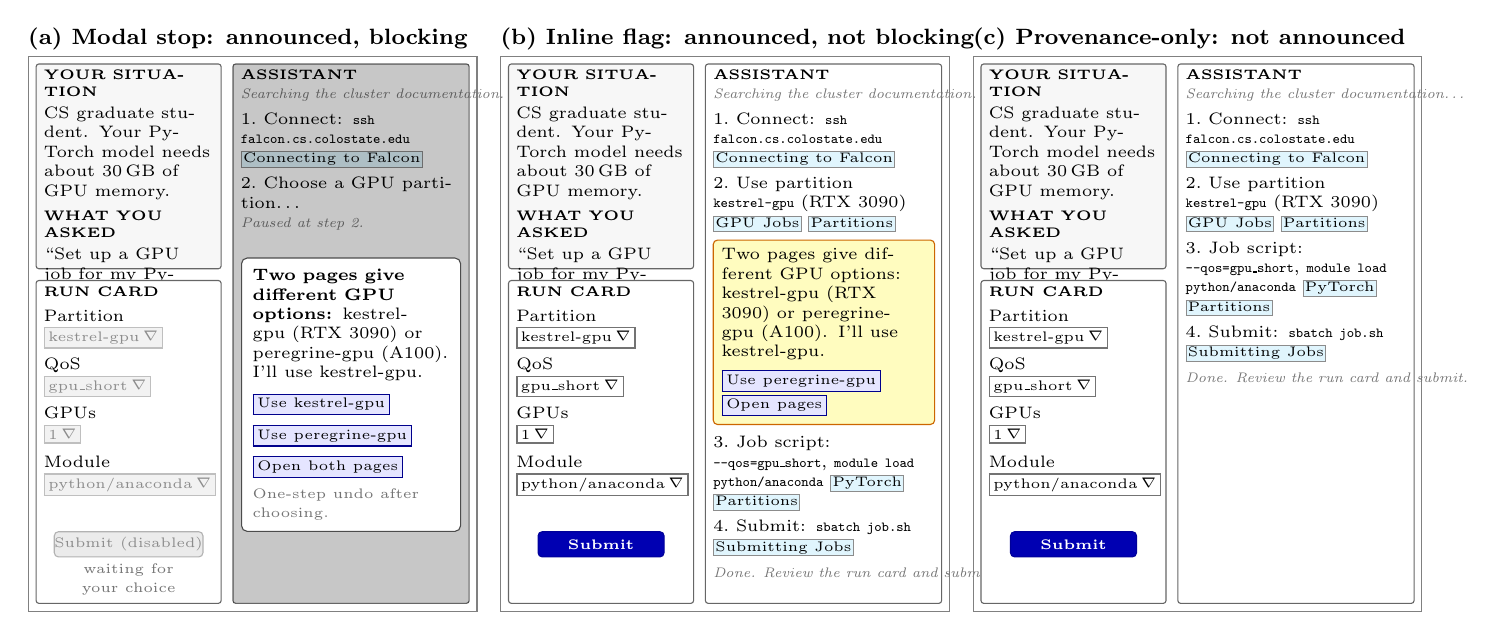
\begin{tikzpicture}[x=1cm, y=1cm, every node/.style={inner sep=0pt, outer sep=0pt, font=\mf}]
% ---- common panel drawing
\newcommand{\basepanel}[2]{% #1 = greyed card (1) or live (0); #2 = label
  \draw[black!50, line width=0.4pt] (0,0) rectangle (5.7,-7.05);
  \node[anchor=south west, font=\footnotesize\bfseries] at (0,0.08) {#2};
  % task card
  \draw[black!60, fill=black!3, rounded corners=1pt] (0.1,-0.1) rectangle (2.45,-2.7);
  \node[anchor=north west, text width=2.15cm, align=left] at (0.2,-0.18)
    {\mfs\textbf{YOUR SITUATION}\\[1pt]\mf CS graduate student. Your PyTorch model needs about 30\,GB of GPU memory.\\[3pt]
     \mfs\textbf{WHAT YOU ASKED}\\[1pt]\mf ``Set up a GPU job for my PyTorch model.''};
  % run card
  \draw[black!60, fill=white, rounded corners=1pt] (0.1,-2.85) rectangle (2.45,-6.95);
  \node[anchor=north west] at (0.2,-2.93) {\mfs\textbf{RUN CARD}};
  \ifnum#1=1
    \node[anchor=north west] at (0.2,-3.22) {\mf Partition};
    \node[anchor=north west] at (0.2,-3.44) {\ddg{kestrel-gpu}};
    \node[anchor=north west] at (0.2,-3.84) {\mf QoS};
    \node[anchor=north west] at (0.2,-4.06) {\ddg{gpu\_short}};
    \node[anchor=north west] at (0.2,-4.46) {\mf GPUs};
    \node[anchor=north west] at (0.2,-4.68) {\ddg{1}};
    \node[anchor=north west] at (0.2,-5.08) {\mf Module};
    \node[anchor=north west] at (0.2,-5.30) {\ddg{python/anaconda}};
    \node[draw=black!30, fill=black!8, rounded corners=1.5pt, minimum width=1.6cm, minimum height=0.32cm] at (1.275,-6.2) {\mfs\color{black!45}Submit (disabled)};
    \node[anchor=north, text width=2.1cm, align=center] at (1.275,-6.45) {\mfs\color{black!55}waiting for your choice};
  \else
    \node[anchor=north west] at (0.2,-3.22) {\mf Partition};
    \node[anchor=north west] at (0.2,-3.44) {\dd{kestrel-gpu}};
    \node[anchor=north west] at (0.2,-3.84) {\mf QoS};
    \node[anchor=north west] at (0.2,-4.06) {\dd{gpu\_short}};
    \node[anchor=north west] at (0.2,-4.46) {\mf GPUs};
    \node[anchor=north west] at (0.2,-4.68) {\dd{1}};
    \node[anchor=north west] at (0.2,-5.08) {\mf Module};
    \node[anchor=north west] at (0.2,-5.30) {\dd{python/anaconda}};
    \node[draw=blue!60!black, fill=blue!70!black, rounded corners=1.5pt, minimum width=1.6cm, minimum height=0.32cm] at (1.275,-6.2) {\mfs\color{white}\textbf{Submit}};
  \fi
  % assistant pane frame
  \draw[black!60, fill=white, rounded corners=1pt] (2.6,-0.1) rectangle (5.6,-6.95);
  \node[anchor=north west] at (2.7,-0.18) {\mfs\textbf{ASSISTANT}};
  \node[anchor=north west] at (2.7,-0.42) {\mfs\itshape\color{black!55}Searching the cluster documentation\ldots};
  \node[anchor=north west, text width=2.8cm, align=left] (s1) at (2.7,-0.72)
    {\mf 1.\ Connect: \mono{ssh falcon.cs.colostate.edu} \chip{Connecting to Falcon}};
}
% ================= panel (a): modal stop
\begin{scope}
\basepanel{1}{(a) Modal stop: announced, blocking}
\node[anchor=north west, text width=2.8cm, align=left, below=1.2mm of s1.south west, anchor=north west] (s2)
  {\mf 2.\ Choose a GPU partition\ldots};
\node[anchor=north west, below=1.2mm of s2.south west, anchor=north west] (pause)
  {\mfs\itshape\color{black!55}Paused at step 2.};
% overlay
\fill[black, fill opacity=0.22] (2.6,-0.1) rectangle (5.6,-6.95);
\node[draw=black!70, fill=white, rounded corners=2pt, text width=2.5cm, align=left, inner sep=4pt] at (4.1,-4.3)
  {\mf\textbf{Two pages give different GPU options:} kestrel-gpu (RTX 3090) or peregrine-gpu (A100). I'll use kestrel-gpu.\\[4pt]
   \btn{Use kestrel-gpu}\\[2.5pt]\btn{Use peregrine-gpu}\\[2.5pt]\btn{Open both pages}\\[3pt]
   \mfs\color{black!55}One-step undo after choosing.};
\end{scope}
% ================= panel (b): inline flag
\begin{scope}[xshift=6.0cm]
\basepanel{0}{(b) Inline flag: announced, not blocking}
\node[text width=2.8cm, align=left, below=1.2mm of s1.south west, anchor=north west] (s2)
  {\mf 2.\ Use partition \mono{kestrel-gpu} (RTX 3090) \chip{GPU Jobs} \chip{Partitions}};
\node[draw=orange!80!black, fill=yellow!25, rounded corners=1.5pt, text width=2.6cm, align=left, inner sep=3pt, below=1mm of s2.south west, anchor=north west] (flag)
  {\mf Two pages give different GPU options: kestrel-gpu (RTX 3090) or peregrine-gpu (A100). I'll use kestrel-gpu.\\[3pt]\btn{Use peregrine-gpu} \btn{Open pages}};
\node[text width=2.8cm, align=left, below=1.5mm of flag.south west, anchor=north west] (s3)
  {\mf 3.\ Job script: \mono{--qos=gpu\_short}, \mono{module load python/anaconda} \chip{PyTorch} \chip{Partitions}};
\node[text width=2.8cm, align=left, below=1.2mm of s3.south west, anchor=north west] (s4)
  {\mf 4.\ Submit: \mono{sbatch job.sh} \chip{Submitting Jobs}};
\node[anchor=north west, below=1.5mm of s4.south west, anchor=north west]
  {\mfs\itshape\color{black!55}Done. Review the run card and submit.};
\end{scope}
% ================= panel (c): provenance-only
\begin{scope}[xshift=12.0cm]
\basepanel{0}{(c) Provenance-only: not announced}
\node[text width=2.8cm, align=left, below=1.2mm of s1.south west, anchor=north west] (s2)
  {\mf 2.\ Use partition \mono{kestrel-gpu} (RTX 3090) \chip{GPU Jobs} \chip{Partitions}};
\node[text width=2.8cm, align=left, below=1.2mm of s2.south west, anchor=north west] (s3)
  {\mf 3.\ Job script: \mono{--qos=gpu\_short}, \mono{module load python/anaconda} \chip{PyTorch} \chip{Partitions}};
\node[text width=2.8cm, align=left, below=1.2mm of s3.south west, anchor=north west] (s4)
  {\mf 4.\ Submit: \mono{sbatch job.sh} \chip{Submitting Jobs}};
\node[anchor=north west, below=1.5mm of s4.south west, anchor=north west]
  {\mfs\itshape\color{black!55}Done. Review the run card and submit.};
\end{scope}
\end{tikzpicture}
\caption{Item G1 at the fork under the three forms (wireframes). In each
panel the left column holds the task card (\emph{Your situation}, seen
only by the participant; \emph{What you asked}, the only input the
assistant received) and the run card (dropdowns pre-selected with the
assistant's choices; only Partition is scored). The center is the
assistant pane; a source panel that opens a cited page with the passage
highlighted sits to its right and is omitted here. Steps, citations,
default and undo are identical; only the rendering of step 2 differs.}
\label{fig:mocks}
\end{figure*}

\subsection{The three forms}
\label{sec:forms}

All three forms share one skeleton: the same steps, the same default, the
same two pages as citations, the same controls (use the other option, open
a page) with one-step undo. This holds MiPP's C1--C3 constant. The forms
are defined by two properties, whether the fork is \emph{announced} and
whether the task is \emph{blocked}: \textbf{modal stop} (announced,
blocking) pauses streaming at the fork step, overlays the sentence with
buttons for both options and \emph{Open both pages}, and disables the card
until a choice is made; \textbf{inline flag} (announced, not blocking)
streams all steps and puts the same sentence with \emph{Use
peregrine-gpu} and \emph{Open pages} on the fork step, card pre-filled,
ignorable; \textbf{provenance-only} (not announced) streams all steps, the
fork step reads ``Use partition kestrel-gpu (RTX 3090)'' with two
citation chips and no warning, and the fork is discoverable only by
opening a page. Figure~\ref{fig:mocks} shows all three for one item. The
forms are not MiPP's families, which also differ in trigger and in whether
the system acts before or after asking; we take MiPP's constraints, not
its taxonomy. Provenance-only is current practice~\cite{ravi2025} and the
C5 silence of Section~\ref{sec:related}. Verification is defined as
opening a diverging page, which no form forces, so a difference cannot be
produced by the modal form requiring a click; the modal form does force a
\emph{choice}, which is inherent to blocking and reported as such.

\subsection{Why this is an agentic, human-centered study}
\label{sec:agentic}

\begin{figure}[t]
\centering
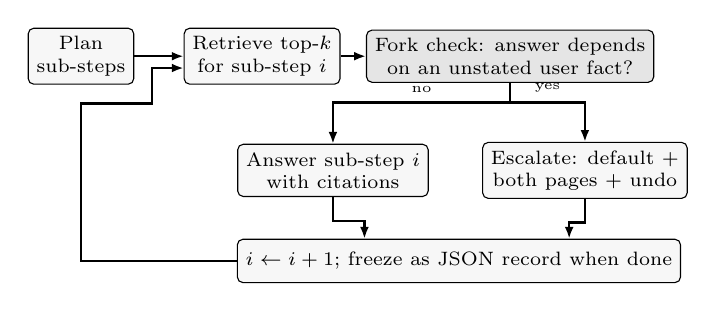
\begin{tikzpicture}[x=1cm, y=1cm,
  box/.style={draw, rounded corners=2pt, align=center, font=\scriptsize,
              minimum height=5.5mm, inner sep=3pt, fill=black!3},
  dec/.style={draw, rounded corners=2pt, align=center, font=\scriptsize,
              minimum height=5.5mm, inner sep=3pt, fill=black!10},
  arr/.style={-{Latex[length=1.5mm]}, thick}
]
\node[box] (plan) at (0,0) {Plan\\sub-steps};
\node[box] (ret) at (2.3,0) {Retrieve top-$k$\\for sub-step $i$};
\node[dec] (chk) at (5.45,0) {Fork check: answer depends\\on an unstated user fact?};
\node[box] (ans) at (3.2,-1.45) {Answer sub-step $i$\\with citations};
\node[box] (esc) at (6.4,-1.45) {Escalate: default $+$\\both pages $+$ undo};
\node[box] (next) at (4.8,-2.6) {$i \leftarrow i+1$; freeze as JSON record when done};
\draw[arr] (plan) -- (ret);
\draw[arr] (ret) -- (chk);
\draw[arr] (chk.south) -- ++(0,-0.25) -| node[above, font=\tiny, pos=0.25] {no} (ans.north);
\draw[arr] (chk.south) -- ++(0,-0.25) -| node[above, font=\tiny, pos=0.25] {yes} (esc.north);
\draw[arr] (ans.south) -- ++(0,-0.3) -| ([xshift=-1.2cm]next.north);
\draw[arr] (esc.south) -- ++(0,-0.3) -| ([xshift=1.4cm]next.north);
\draw[arr] (next.west) -| (0,-1.45) -- (0,-0.6) -- (0.9,-0.6) |- ([yshift=-1.5mm]ret.west);
\end{tikzpicture}
\caption{The loop that drafts each item. The fork check is the
retrieval-score margin plus an LLM judge. Its output is frozen and replayed
identically to every participant; only the rendering of the ``Escalate''
step differs between conditions.}
\label{fig:loop}
\end{figure}

Items are drafted by a minimal agentic RAG loop (Figure~\ref{fig:loop}):
given the question it plans sub-steps, retrieves the top-$k$ chunks per
sub-step from the snapshot, and runs a fork check that fires when the
retrieval-score margin
between the top candidates is small \emph{and} an LLM judge answers yes to
``do these chunks give different answers depending on a user attribute the
question does not state?'' Only items on which the check fired become
flagged items; we report its hit rate. Each item is then frozen as a JSON
record (situation, question, steps with citations, fork step index,
options, default, card fields with options and pre-fill, scored field,
key), and the web app reads only the record, so every participant sees
identical content and the condition flag changes only the fork step's
rendering.

\emph{Pre-generated, replayed behavior.} Agent behavior is generated by the
pipeline before the sessions and replayed identically to every participant,
following the fixed-advice paradigm common in AI-reliance
studies~\cite{bucinca2021,vasconcelos2023,schemmer2023}\verify{} and the
older practice of controlling system behavior in intelligent-interface
studies~\cite{dahlback1993}\verify{}, so that escalation points, defaults
and default correctness are controlled. The pipeline runs locally on an
open-weight model at temperature 0 with a fixed seed; snapshot, records and
model digests are released. Authors may edit wording but never an
escalation decision or a default; default correctness is set by the
situation line. Participants are told responses were prepared in advance.
The study thus isolates the human-facing form of an agent-initiated
escalation, not the agent's behavior or multi-turn interaction. This passes the ``if a
chatbot can do it'' test: a chatbot answers the question as asked, and
only a loop that retrieves per step and inspects its own retrieval can
discover mid-task that the answer depends on an unstated fact and choose to
hand the decision back. The human-centered question is what that hand-back
should look like, and every outcome is a human behavior. ``Agentic'' rests
on four properties, each verifiable in the released records: the task is
multi-step, the escalation arrives at the affected step, the trigger is the
loop's own decision, and the loop is fully described here.

\subsection{Corpus and items}
\label{sec:corpus}

% Corpus selection is not final. Requirements below are fixed.
The corpus is drawn from the CSU CS department systems documentation
(sna.cs.colostate.edu); which sections are used is not yet decided.
Requirements are fixed: a frozen snapshot; every key derivable from the
snapshot plus the situation line, with no administrator verification;
snapshot and item records released together; 18 measured items (12
flagged, 6 control) plus 2 practice items from three disjoint sections
(for example GPU and jobs, access and remote connection, storage and
software); and a system many CSU students have not used.
Table~\ref{tab:items} gives illustrative items written against the current
pages. We keep the FictionalQA blind-versus-informed
check~\cite{kirchenbauer2026} as a filter: the drafting model is queried
blind and with the two pages, and facts it answers correctly blind are
discarded (department-local hostnames, partition names and paths are the
kind that fail blind). Task sets are matched on number of steps, number of
card fields, question--page lexical overlap band, fork type and fork
position, checked in the pilot, and item is a random effect in every model.
Because someone who knows that a 3090 has 24\,GB could resolve G1 without
opening a page, we screen for prior use, prefer items whose condition is
stated only on the page, and log what was opened.

\begin{table}[t]
\centering\scriptsize
\caption{Illustrative items from the CSU CS systems documentation. Only the
scored field is compared with the key. G2 is default-correct; C1 is a
control item. Page facts are from the current pages; the exact pairing is
illustrative until the snapshot is frozen.}
\label{tab:items}
\begin{tabular}{@{}>{\raggedright\arraybackslash}p{0.04\linewidth}>{\raggedright\arraybackslash}p{0.27\linewidth}>{\raggedright\arraybackslash}p{0.36\linewidth}>{\raggedright\arraybackslash}p{0.17\linewidth}@{}}
\toprule
\textbf{ID} & \textbf{Your situation / what you asked} & \textbf{Pages and options (scored field)} & \textbf{Default $\rightarrow$ key} \\
\midrule
G1 & Model needs about 30\,GB of GPU memory. ``Set up a GPU job for my PyTorch model.'' & GPU Jobs, Partitions: \texttt{kestrel-gpu} (RTX 3090, 24\,GB each) vs.\ \texttt{peregrine-gpu} (A100, 40/80\,GB). Field: partition. & kestrel-gpu (wrong) $\rightarrow$ peregrine-gpu \\
\addlinespace
G2 & Model fits in 16\,GB. Same question. & Same pages and field. & kestrel-gpu (correct) \\
\addlinespace
R1 & Working from home. ``How do I connect to Falcon?'' & Connecting to Falcon: \texttt{ssh falcon.cs.colostate.edu}; SSH guide: off campus, connect to the CSU VPN first. Field: first step. & ssh directly (wrong) $\rightarrow$ VPN, then ssh \\
\addlinespace
S1 & Output is scratch data you can regenerate. ``Where should my job write its output?'' & Home Directories: home (backed up, quota); Temporary Disk Space: \texttt{/s/<host>/a/tmp} (not backed up, scrubbed). Field: output path. & home (wrong) $\rightarrow$ \texttt{/s/<host>/}\allowbreak\texttt{a/tmp} \\
\addlinespace
C1 & (none) ``Why is my job still pending?'' & FAQ and Monitoring Jobs agree: \texttt{squeue}, REASON column. No fork. Field: command. & squeue (correct) \\
\bottomrule
\end{tabular}
\end{table}

\section{System Vision and Technology}
\label{sec:vision}

The apparatus is one web application (React or plain JavaScript) with a
condition flag, run in a desktop browser with no headset or spatial
component. The screen has three panes: task card and run card on the
left, the assistant pane in the center, and a source panel on the right
that opens a cited page with the relevant passage highlighted
(Figure~\ref{fig:mocks}). A replay engine reads the item's JSON record and
streams it at a fixed pace; the flag selects one of three renderings of
the fork step and nothing else. Every interaction is logged as a
timestamped event (item, condition, fork onset, each control used, each
page opened and for how long, each dropdown change, the submitted card,
block boundaries) to a local SQLite database under a participant code.
Instruments appear as full-screen steps between blocks. The drafting
pipeline is Python: the snapshot is chunked by heading, embedded into a
vector index, and queried per sub-step; one LLM plans sub-steps and acts
as the fork judge. The model will be named in the paper; because records
are frozen, the human-facing study does not depend on it. We estimate one
week for the pipeline and two for the web application.

\section{Evaluation Plan}
\label{sec:eval}

\paragraph{Design and participants.}
Independent variables: escalation form (modal, inline, provenance-only),
within subjects; and default correctness at flagged items (correct,
wrong), within block. A $3\times3$ Latin square of task set and form with
all six orders; $N{=}18$ target (three per order), 12 minimum; pilot of
3--4. A between-subjects design would need roughly three times as many
people for the same power, which at class scale leaves four to six per
condition, so we keep within subjects. Participants are CSU students who
have not used the documented system (screening item), recruited through
the class data-collection form; the realistic pool is upper-division
undergraduates and new graduate students. The class form suffices for the
course; if we intend to publish, an IRB protocol with a faculty principal
investigator is needed before recruitment, and we will raise it with the
instructor in the first two weeks of October.

\paragraph{Procedure.}
A session takes about 45 minutes: consent and instructions, which tell
everyone that the assistant is usually right but can be wrong (5 min); a
two-item practice block without forks (3 min); three measured blocks of
six items (4 flagged, 2 default-correct and 2 default-wrong, plus 2
control; order randomized within block), each followed by raw NASA-TLX and
one perceived-intrusion item (about 9 min per block); and a closing
questionnaire with a manipulation check (identify the form just used), a
ranking of the three forms and a free-text reason (5 min). Every critical
fact appears in exactly one item and task sets come from disjoint
sections; generic steps such as connecting recur but are never scored.
Block position enters the models as a covariate and the first block is
reported alone as a descriptive between-subjects check.

\paragraph{Hypotheses and measures.}
\textbf{H1 (verification):} on flagged items the proportion of items on
which a diverging page is opened before submission is ordered modal $>$
inline $>$ provenance-only. \textbf{H2 (appropriate reliance):}
correcting a wrong default is higher under modal and inline than under
provenance-only, while keeping a correct default does not differ, i.e., a
form $\times$ default-correctness interaction on the scored decision.
\textbf{H3 (cost):} time per flagged item and NASA-TLX per block are
ordered modal $>$ inline $>$ provenance-only. H1 and H3 together are the
trade-off reported for forcing functions~\cite{bucinca2021}; H2 is what
matters to a designer. Measures are: verified; the scored-field decision
crossed with default correctness, from which relative AI reliance and
relative self-reliance follow~\cite{schemmer2023}; time from item onset to
submission; raw NASA-TLX per block; one perceived-intrusion item per block
(1--7, as in MiPP-Eval, for comparability); the manipulation check; and
the ranking with its reason. Nothing else is collected. The ranking is
reported descriptively.

\paragraph{Analysis.}
Primary analyses are at the trial level (four flagged items per condition
per participant): logistic mixed models for verified and for the scored
decision, with fixed effects of form, default correctness, their
interaction and block position, and random intercepts for participant and
item; a linear mixed model on log time; repeated-measures ANOVA with
Greenhouse--Geisser correction, or Friedman, for TLX and intrusion.
Planned contrasts (modal vs.\ inline, inline vs.\ provenance-only) are
Holm-corrected and reported as odds ratios or $d_z$ with 95\% CIs.
Free-text reasons are coded thematically by both authors. A paired
$t$-test at $N{=}12$ detects only large participant-level effects ($d_z
\approx 0.9$ at 80\% power), which is why trial-level models are primary;
we will simulate power for the H2 interaction from pilot estimates.

\paragraph{Threats.}
Strategy carry-over (learning that pages can disagree) is addressed by the
up-front instruction, all six orders, the position covariate and the
first-block check. Domain knowledge that resolves a fork without opening a
page is addressed by screening, item selection and logs. Forced choice
under modal is inherent to blocking; verification is a never-forced act.
Generality is limited to one corpus, novices, a short lab session and
replayed single-turn sessions without follow-up questions, and is stated
as a scope condition.

\section{Deliverables}
\label{sec:deliverables}

\textbf{By mid-November:} the frozen snapshot of the chosen sections; the
drafting pipeline with its fork check and a log of where it fired over
about 30 candidate questions; the contamination-filter survivor count; 18
measured and 2 practice item records assembled into three matched task
sets; the web application with the three renderings, replay engine,
instruments and event logging; a completed pilot of 3--4 people with items
and timing revised; and the IRB decision. \textbf{By the early-December
presentations:} 12--18 completed sessions; the analysis scripts and
results for H1--H3; a paper draft with Method and Results; a demo video of
one item in all three forms; and the released snapshot plus item records.
The critical path is item authoring, not code.

\textbf{Team.} Group CS567\_Coen\_Cam\_Context\_Not\_Found. Coen Petto:
study design, web application and participant sessions. Cameron Suess:
drafting pipeline, item authoring and corpus snapshot. Both authors write
and analyze.
% TODO authors: confirm roles

\section{Conclusion}

We propose a within-subjects study of how an agentic RAG assistant should
hand back a decision that depends on a fact about the user it was never
told. Only the form varies. The prediction is that a modal
stop buys the most verification at the highest cost, that an inline flag
captures most of the benefit for less, and that a provenance-only cue,
which is what current RAG interfaces provide and what MiPP's C5 counsels,
leaves the agent's errors largely uncaught.

\section*{Use of AI}

Claude Code (Anthropic), running Claude Opus 5.5 with Claude Fable 5.1
subagents, was used to critique the proposal, check claims against MiPP,
check references against publisher records, draft this text and draw the
mock-ups. The authors made every design decision, revise the text and
verify each reference; claims still to be checked are marked \verify.
% TODO authors: verify -- add any other AI tools used on the original
% proposal (for example, for grammar or LaTeX fixes) and what each did.

%% ---------------------------------------------------------------- references
\bibliographystyle{ACM-Reference-Format}
\bibliography{references}

\end{document}
